\documentclass[a4paper]{article}
\usepackage[english]{babel}
\usepackage[a4paper,top=2cm,bottom=2cm,left=2cm,right=2cm,marginparwidth=1.75cm]{geometry}
\usepackage{amsmath}
\usepackage{amsfonts}
% \usepackage{amsthm}
\usepackage{amssymb}
\usepackage{graphicx}
\usepackage[colorinlistoftodos]{todonotes}
\usepackage[colorlinks=true, allcolors=blue]{hyperref}
\usepackage{import}
\usepackage{pdfpages}
\usepackage{transparent}
\usepackage{xcolor}
\usepackage{algorithmicx}
\usepackage{algpseudocode}
\usepackage{hyperref}

\usepackage{thmtools}
\usepackage{enumitem}
\usepackage[framemethod=TikZ]{mdframed}

\usepackage{xpatch}

\usepackage{boites}
\makeatletter
\xpatchcmd{\endmdframed}
{\aftergroup\endmdf@trivlist\color@endgroup}
{\endmdf@trivlist\color@endgroup\@doendpe}
{}{}
\makeatother

%\usepackage[poster]{tcolorbox}
%\allowdisplaybreaks
%\sloppy

\usepackage[many]{tcolorbox}

\xpatchcmd{\proof}{\itshape}{\bfseries\itshape}{}{}

% to set box separation
\setlength{\fboxsep}{0.8em}
\def\breakboxskip{7pt}
\def\breakboxparindent{0em}

\newenvironment{proof}{\begin{breakbox}\textit{Proof.}}{\hfill$\square$\end{breakbox}}
\newenvironment{ans}{\begin{breakbox}\textit{Answer.}}{\end{breakbox}}
\newenvironment{soln}{\begin{breakbox}\textit{Solution.}}{\end{breakbox}}

% \tcolorboxenvironment{proof}{
%     blanker,
%     before skip=\topsep,
%     after skip=\topsep,
%     borderline={0.4pt}{0.4pt}{black},
%     breakable,
%     left=12pt,
%     right=12pt,
%     top=12pt,
%     bottom=12pt,
% }
%
% \tcolorboxenvironment{ans}{
%     blanker,
%     before skip=\topsep,
%     after skip=\topsep,
%     borderline={0.4pt}{0.4pt}{black},
%     breakable,
%     left=12pt,
%     right=12pt,
% }

\mdfdefinestyle{enclosed}{
    linecolor=black
    ,backgroundcolor=none
    ,apptotikzsetting={\tikzset{mdfbackground/.append style={fill=gray!100,fill opacity=.3}}}
    ,frametitlefont=\sffamily\bfseries\color{black}
    ,splittopskip=.5cm
    ,frametitlebelowskip=.0cm
    ,topline=true
    ,bottomline=true
    ,rightline=true
    ,leftline=true
    ,leftmargin=0.01cm
    ,linewidth=0.02cm
    ,skipabove=0.01cm
    ,innerbottommargin=0.1cm
    ,skipbelow=0.1cm
}

\mdfsetup{%
    middlelinecolor=black,
    middlelinewidth=1pt,
roundcorner=4pt}

\setlength{\parindent}{0pt}

\mdtheorem[style=enclosed]{theorem}{Theorem}
\mdtheorem[style=enclosed]{lemma}{Lemma}[theorem]
\mdtheorem[style=enclosed]{claim}{Claim}[theorem]
\mdtheorem[style=enclosed]{ques}{Question}
\mdtheorem[style=enclosed]{defn}{Definition}
\mdtheorem[style=enclosed]{notn}{Notation}
\mdtheorem[style=enclosed]{obs}{Observation}
\mdtheorem[style=enclosed]{eg}{Example}
\mdtheorem[style=enclosed]{cor}{Corollary}
\mdtheorem[style=enclosed]{note}{Note}

% \let\thetheorem=\relax
% \let\thelemma=\relax
% \let\theclaim=\relax
% \let\theques=\relax
% \let\thedefn=\relax
% \let\thenotn=\relax
% \let\theobs=\relax
% \let\thecor=\relax
% \let\thenote=\relax

% \renewcommand\qedsymbol{$\blacksquare$}
\newcommand{\nl}{\vspace{0.2cm}\\}
\newcommand{\ol}{\overline}
\newcommand{\eps}{\varepsilon}
\newcommand{\mc}{\mathcal}
\newcommand{\mi}{\mathit}
\newcommand{\mf}{\mathbf}
\newcommand{\mb}{\mathbb}
\newcommand{\R}{\mathbb{R}}
\newcommand{\Z}{\mathbb{Z}}
\newcommand{\OPT}{\mathbf{OPT}}
\newcommand{\ALG}{\mathbf{ALG}}
\renewcommand{\L}{\mc{L}}
\newcommand{\changesto}{\vdash}
\newcommand\Vtextvisiblespace[1][.3em]{%
    \mbox{\kern.06em\vrule height.3ex}%
    \vbox{\hrule width#1}%
    \hbox{\vrule height.3ex}
}
\newcommand{\blank}{{\Vtextvisiblespace[0.7em]}}
\newcommand{\leftend}{\triangleright}
\newcommand{\comp}{\overline}

\newcommand{\incfig}[1]{%
    \def\svgwidth{\columnwidth}
    \import{./figures/}{#1.pdf_tex}
}
\pdfsuppresswarningpagegroup=1

\title{\textbf{ELL888 Minor Exam}}
\author{Navneel Singhal, 2018CS10360}
\date{}

\begin{document}

\maketitle
\tableofcontents

\setcounter{section}{-1}

\section{Graph learning setting}

You are given $\mf{X} \in \R^{n \times d}$ whose rows reside on the vertices of an unknown graph.
\begin{align*}
    X = \begin{bmatrix}
        - \mf{x}_1 \in \R^d -\\
        - \mf{x}_2 \in \R^d -\\
            \mid \\
        - \mf{x}_n \in \R^d -\\
    \end{bmatrix}
\end{align*}
Graph learning from data simply means finding an edge-weight matrix $\mf{A} \in \R^{n \times n}$ where its element $w_{ij} = {[A]}_{ij}$ captures the relation between any two pairs of vertices $(i,
j)$, i.e., data points $(\mf{x}_i, \mf{x}_j)$. We learn the graph weights $\mf{w} \in \R^{n(n - 1)/2}$ under certain assumptions like smoothness, probabilistic distribution, nearest
neighbourhood, etc. The focus here is an undirected graph which implies that the graph matrix is symmetric. Now consider the following problems.

\section{Graph learning with missing data}

\subsection{Problem}
\begin{align*}
    X = \begin{bmatrix}
        \mf{x}_1 = [x_{11}, x_{12}, \bullet, x_{14}, \ldots, x_{1d}]\\
        \mf{x}_2 = [x_{21}, \bullet, x_{23}, \bullet, x_{25}, \ldots, x_{1d}]\\
        \mid\\
        \mf{x_n} = [\bullet, x_{n2}, \bullet, x_{n4}, \ldots, x_{nd}]
    \end{bmatrix}
\end{align*}
where some parts of the data are missing at random and $\bullet$ indicates missing data. Explain in detail how we can learn the graph matrix with missing data (in descriptive detail).

\subsection{Solution}
I will mainly focus on solving this problem under smoothness constraints --- i.e., I will assume that we want to learn a graph from a smooth signal.

\subsubsection{Optimization problem formulation}
Firstly, note that a rudimentary imputation scheme is to do the following: for each feature $i \in \{1, \ldots, d\}$, let $D$ be the distribution of the values for the feature that are not
missing. Then, for each $x_i$ such that $x_{id}$ is a missing feature, assign to it a value sampled from $D$. We could also assign it something different --- for instance, the mean of $D$.\nl
However, this is clearly not good enough. Let's look at the formulation of the optimization problem for the weights $\mf{w}$ (with $w(i, j)$ corresponding to the weight of the edge between
$i$ and $j$). It looks something like the following:\\
\begin{align*}
    \min_{w} \sum_{1 \le i < j \le n} w(i, j) ||\mf{x}_i - \mf{x}_j||_2^2\\
    \text{subject to certain constraints on }w
\end{align*}
Note that we are working under the assumption that the signal is smooth. Considering the fact that in graph regularization, such an ``energy'' term is used to penalize the objective function, it
makes sense to consider the above problem as a minimization problem when we vary the missing data as well, so as to ensure that the graph signal is indeed smooth. That is, the problem transforms to the following:

\begin{align*}
    \min_{w, x_{\text{unknown}}} \sum_{1 \le i < j \le n} w(i, j) ||\mf{x}_i - \mf{x}_j||_2^2\\
    \text{subject to certain constraints on }w
\end{align*}

In a sense, alongside the weights $\mf{w}$, we are also learning the missing data under the smoothness assumption.

\subsubsection{Solving the optimization problem}
For solving this optimization problem, we can follow the following iterative method to solve for optimal $w, x_{\text{unknown}}$ given that we have a solver for the original problem as a
black-box (in certain special cases, it is possible to solve this directly rather than relying on the following distribution):

\begin{enumerate}
    \item For each feature $j \in \{1, \ldots, d\}$, compute the multiset $D_j$ of values that appear in $\mf{X}$, and for each $\mf{x}_i$ such that $x_{ij}$ is missing, assign
        to $x_{ij}$ a random sample from $D_j$ (or the mean).
    \item Until a stopping condition is reached, do the following:
        \begin{itemize}
            \item Keeping $x_{\text{unknown}}$ fixed, solve the optimization problem for $\mf{w}$ using the black-box algorithm.
            \item Keeping $\mf{w}$ fixed, solve the quadratic programming problem for $x_{\text{unknown}}$ to get an optimal solution $x^*_{\text{unknown}}$.
        \end{itemize}
    \item Return the learned weights $\mf{w}$.
\end{enumerate}

Here, the first step tries to learn $\mf{w}$ using our prior beliefs about the unknown data, and later on, we try to refine the unknown data by performing some sort of regularization of the
graph signal in order to fit it to a more regular signal.\nl

Note that if a fraction $k$ of the data was missing, then in the quadratic programming problem that we need to solve, there would be $knd$ variables, which might be infeasible for a
large number of variables. A variant of the above method would be to optimize over these unknown variables in batches (similar to stochastic gradient descent) while keeping the other variables
constant, so as to make the size of this problem small enough.

\subsubsection{Experiment}
Firstly, a comment on the applicability of this method: note that in the mentioned algorithm, we assumed that we only have access to an oracle that learns weights from a graph (and it is called in
the second part of the loop in our algorithm). Hence, this method is applicable for practically any scenario where we want to learn the weight matrix from data, no matter what the constraints
on $\mf{w}$ that the oracle provides, or the form of the objective function (though if the dependence of the objective function on $x$ is not quadratic, it becomes a different problem ---
however, the idea remains the same). However, it is not clear if the convergence is guaranteed.\nl
To benchmark it, we shall use the approach in the following paper for the aforementioned oracle:

\begin{itemize}
    \item Dong et al. ``Laplacian Matrix Learning for Smooth Graph Signal Representation''. ICASSP, 2015.
\end{itemize}

Since our objective at hand is to see how well the imputed data represents the original data had it not been missing, we shall take the following approach:
\begin{itemize}
    \item Take a dataset $X$ of complete data, and remove a certain fraction of values to get a new dataset $X'$.
    \item Using the oracle $\mc{O}$, compute the graph $G$, and using our algorithm, compute the graph $G'$ and the dataset $X''$ consisting of new values.
    \item Compute the difference between $X$ and $X''$ on the imputed parts for each feature, and find the average square of the difference between the actual data and imputed data for each
        feature.
    \item Compare the F-measures of edge existence.
\end{itemize}

Since we are working under the assumption that the graph signal is smooth, we will choose the following dataset:

\begin{itemize}
    \item Randomly generated sensor networks: Since sensor networks aim to measure some physical property, which should be reasonably smooth, these graphs are good candidates for this approach.
        The graph signal is generated by embedding these sensors in 2D and applying smooth functions to their coordinates.
\end{itemize}

The implementation uses the base code found at \href{https://github.com/rodrigo-pena/graph-learning}{https://github.com/rodrigo-pena/graph-learning}, and it was retrieved from
\href{https://paperswithcode.com/paper/how-to-learn-a-graph-from-smooth-signals}{https://paperswithcode.com/paper/how-to-learn-a-graph-from-smooth-signals}. Some of the metrics that we
want are already implemented there, but we will are also using some new metrics and they are self-implemented. The code author has released it for public use, and the license is included with the code in the code
directory.\nl

\subsubsection{Results}

For the following experiments, we have $n = 256, d = 4$. In the baseline, we assign the mean of the feature to the missing values. We use $k = 0.05$ and $k = 0.1$ (i.e., $5\%$ and $10\%$ of data
missing respectively) in two independent sets of experiments to show the differences between this and the baseline.

Define $$\ell_j = \sqrt{\frac{\sum_{i = 1}^n (x_{ij} - x_{ij, \text{imputed}})^2}{\sum_{i = 1}^n 1_{x_{ij}\text{ is missing}}}}$$

and
$$
\omega = \frac{||W_{full} - W_{imputed}||_F^2}{n \times d}
$$

Then we have the following

\begin{center}
\begin{tabular}{|c|c|c|c|}
    \hline
                                & Baseline  & Our algorithm     & No missing data \\
    \hline
    F2-score at $k = 0.05$      & 0.60      & 0.67              & 0.70 \\
    \hline
    F2-score at $k = 0.1$       & 0.49      & 0.61              & 0.69 \\
    \hline
    $\omega$ at $k = 0.05$      & 0.0165    &    0.0118         & ---\\
    \hline
    $\omega$ at $k = 0.1$       & 0.0357    &    0.0223         & ---\\
    \hline
    $\ell_1$ at $k = 0.05$      & 1.156     &    0.833          & ---\\
    \hline
    $\ell_2$ at $k = 0.05$      & 4.033     &      3.894          & ---\\
    \hline
    $\ell_3$ at $k = 0.05$      & 1.875     &      1.715        & ---\\
    \hline
    $\ell_4$ at $k = 0.05$      & 0.971     &      0.5712        & ---\\
    \hline
    $\ell_1$ at $k = 0.1$       & 1.359     &    0.956         & ---\\
    \hline
    $\ell_2$ at $k = 0.1$       & 2.558     &   2.1034           & ---\\
    \hline
    $\ell_3$ at $k = 0.1$       & 1.778     &    1.745         & ---\\
    \hline
    $\ell_4$ at $k = 0.1$       & 0.910     &    0.770          & ---\\
    \hline

\end{tabular}
\end{center}

\begin{center}
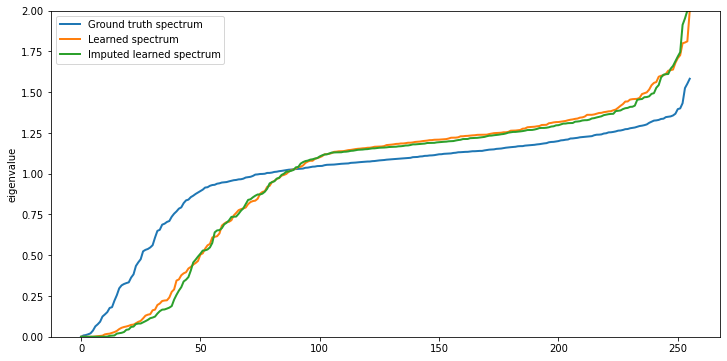
\includegraphics[width=0.70\textwidth]{images/p1/5_percent_own_spectrum.png}\\
Spectrum for $k = 0.05$\\
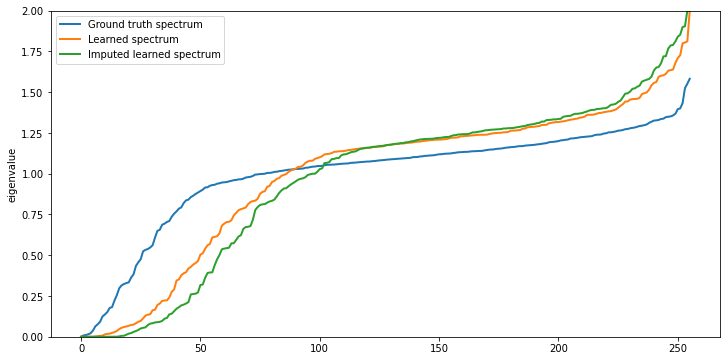
\includegraphics[width=0.70\textwidth]{images/p1/5_percent_baseline_spectrum.png}\\
Baseline spectrum for $k = 0.05$\\
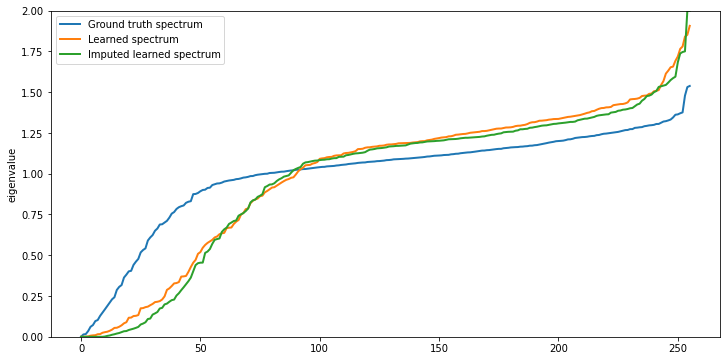
\includegraphics[width=0.70\textwidth]{images/p1/10_percent_own_spectra.png}\\
Spectrum for $k = 0.1$\\
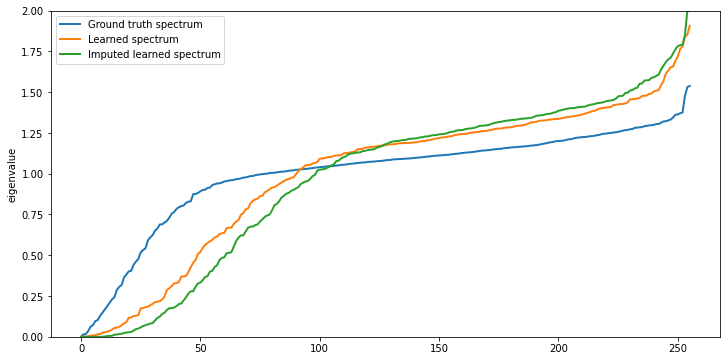
\includegraphics[width=0.70\textwidth]{images/p1/10_percent_baseline_spectra.png}\\
Baseline spectrum for $k = 0.1$\\
\end{center}

As we can see in the above plots of the eigenvalues, our algorithm matches the eigenvalues fairly well.

Now we will show how the learned graphs look like (for $k = 0.1$, baseline and our algorithm respectively):

\begin{center}
    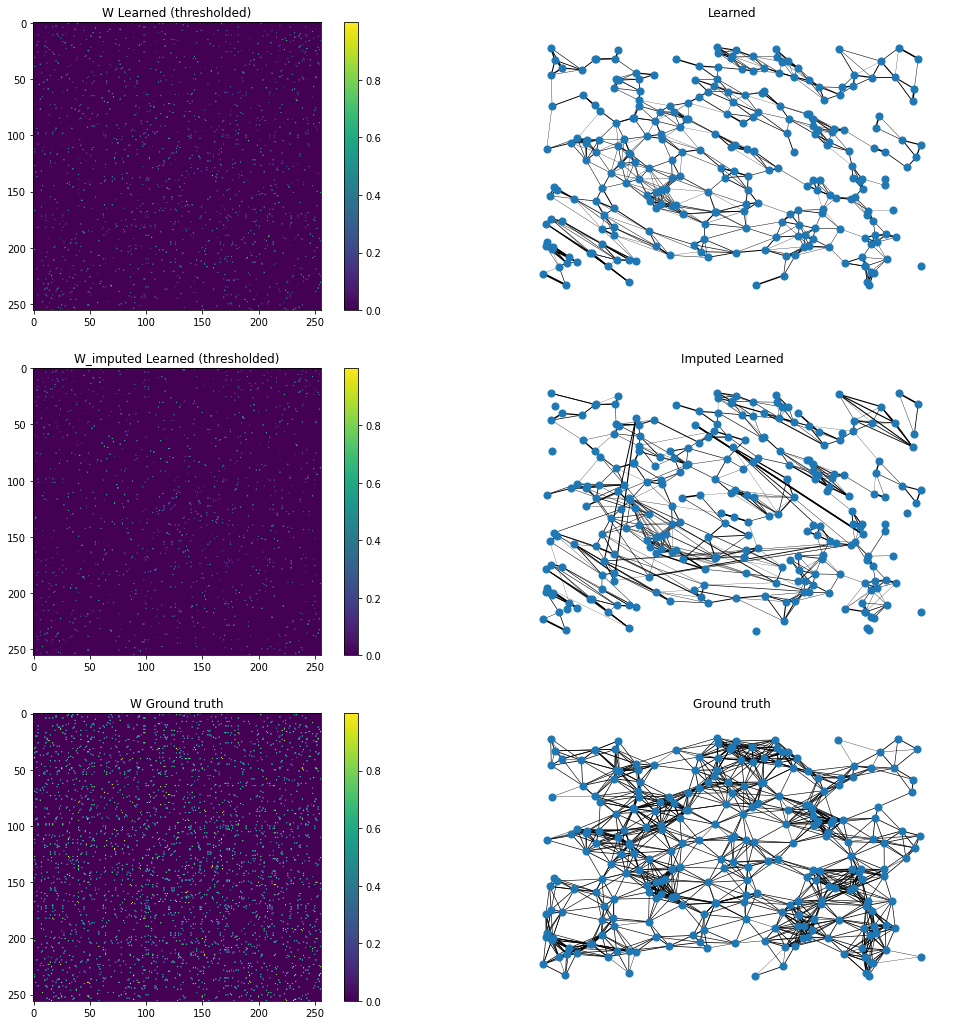
\includegraphics[width=0.45\textwidth]{images/p1/10_percent_baseline_learned_graphs.png}
    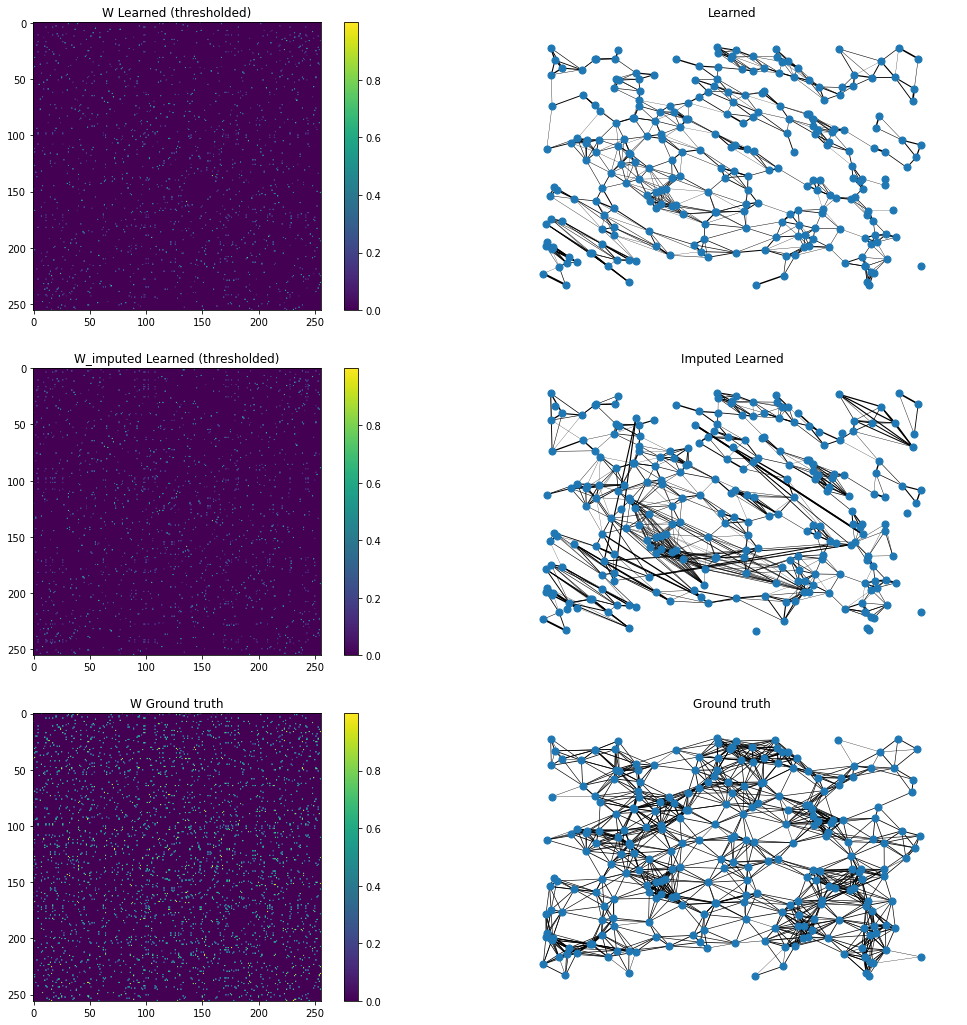
\includegraphics[width=0.45\textwidth]{images/p1/10_percent_own_learned_graphs.png}
\end{center}

Some notable differences in the above figures are how our algorithm learns the far-above-far-left, far-above-middle, below-left and middle-slight-left structures in a manner close to the algorithm without imputed data.

\newpage

\section{Semi-supervised setting}

\subsection{Problem}

Now consider a semi-supervised graph learning problem. With the data $\mf{X}$ sitting at $n$ vertices, we also have the label information for $k < n$ vertices. Simply, we have $\mf{X} \in \R^{n \times
d}$ with label information for $k$ vertices $\mf{y} \in \{0, 1\}^k$. Explain in detail how can we learn the graph matrix integrating the label information. The dataset available is
$\left(\{\mf{x}_i, y_i\}_{i = 1}^k, \{\mf{x}_j\}_{j = k + 1}^n\right)$.

\subsection{Solution}

For this problem, the first idea is to enforce that $w_{ij} = 0$ for vertices $v_i, v_j$ with different labels. An alternate view of this is to penalize the $w_{ij}$ for such vertices
with a regularization term in the form of, for example, altering the pairwise distance matrix of the node data (setting the distance to some large constant), rather than forcing the $w_{ij}$ to be $0$, since that will lead to a more
flexible model in general; both in terms of being easy to incorporate in usual graph learning techniques, as well as being applicable to the (perhaps rare) case where we do not want to predict the labels themselves and
need to learn the graph structure only (i.e., in the case that reconstructing labels might not be the task that we need the graph for). This is equivalent to the following: we construct a graph with
three parts: the part with all vertices having pre-assigned label $0$, another part with all vertices with pre-assigned label $1$, and the final part with vertices whose labels we don't know. As the
penalties on the edges between part $1$ and part $2$ tends to $\infty$, the learned graph tends to a graph where there are no edges between parts $1$ and $2$.\nl
A more sophisticated method would be to do the following iteratively (with increasing penalties $\to \infty$ and decreasing $r \to 1$): after learning this graph, for each unlabelled vertex, compute
the average weight of edges between this vertex and all vertices with label $0$, and similarly the average weight of edges between this vertex and all vertices with label $1$. If the ratio between
the larger of these to the smaller of these exceeds $r$, assign the label corresponding to the smaller average weight to this vertex, and otherwise leave it unlabelled. Do this while
there is at least one vertex that is not assigned.
We can ensure that at least one vertex is classified in each iteration (to ensure termination) by taking replacing $r$ with the minimum of $r$ and the minimum ratio at this step, apart from the
update on $r$ (we can speed this up by ensuring that we choose multiple vertices at each step rather than just one vertex).\nl
A large penalty would lead to a more pronounced difference between the sets of vertices, however it would also unnecessarily give a lot of weightage to the label information if it were to be
used at a point in time when we don't have a sufficiently large set of labelled points. Hence we will use a large penalty only when there is a small number of vertices whose label information is not
available. In any case, if we really want to learn the labels of the graph, we can always put an infinite penalty by enforcing certain $w_{ij}$'s to be zero, which is incidentally what we will be
doing in the example.

\subsubsection{Experiment}

In this example, we will look at how a graph with two clusters can be learnt via this method. The metric would be somewhat indirect, since there is no obvious metric in this case for seeing how well the graph is
learnt apart from looking at how well the labels are predicted using the algorithm.\nl
Hence we will consider a semi-supervised binary node classification problem in a transductive setting.

We will look at varying values of $k$, and do the following comparisons:

\begin{enumerate}
    \item For some subset (of varying sizes) of the nodes, incorporate the label information into the graph learning as explained above as well as learn the graph without incorporating the
        label information, and compare certain metrics of the classification phase on these learned graphs.
    \item For these subsets, also compare the metrics on the labels that we have learnt.
\end{enumerate}

For this, we will use a two-step method: firstly the graph learning (which is our main objective), and then a node-classification algorithm (like label propagation) in a semi-supervised setting (using the original labels).\nl
To this end, the pipeline will look like this:
\begin{enumerate}
    \item For a given graph, use the same algorithm used in problem 1 to learn the graph.
    \item Run label propagation on the learned graph to find the labels.
\end{enumerate}
The dataset would again be synthetically generated as in problem 1.\nl
The same acknowledgement of code as done in question 1 holds here too.
We shall use the two-moons dataset for classification.\nl

Now we show what happens for $k = 0.05, 0.1$ and $0.2$ respectively.

\subsubsection{Results}

The data is as shown:\nl
\begin{center}
    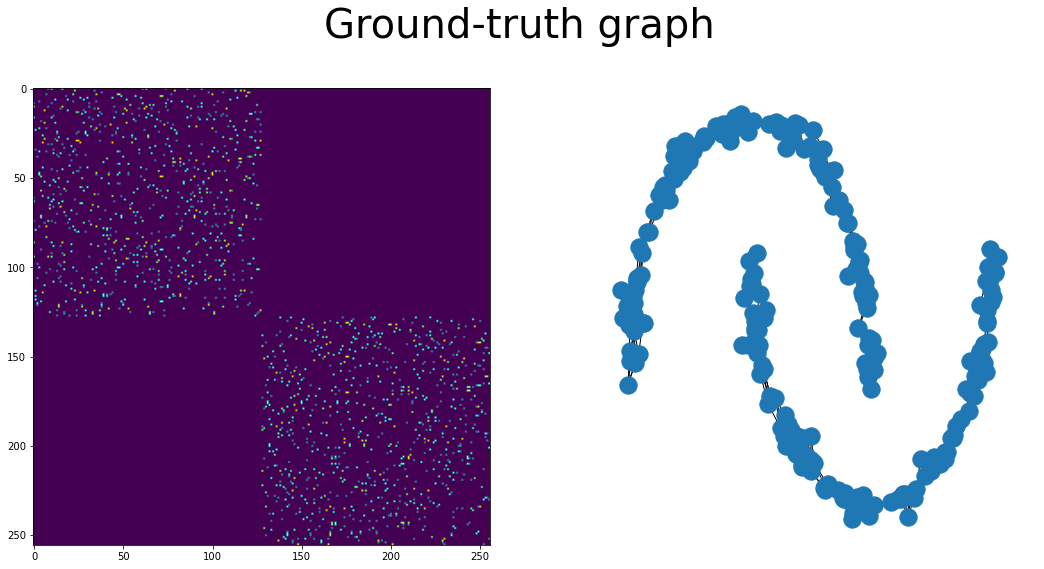
\includegraphics[width=0.5\textwidth]{images/p2/ground_truth.png}\nl
    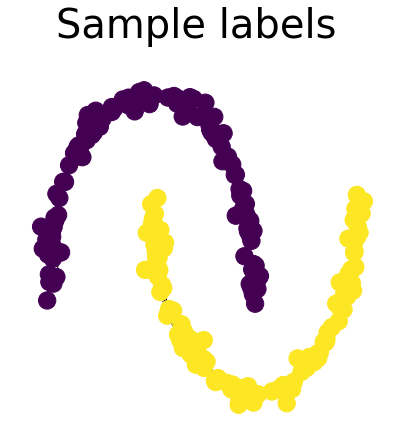
\includegraphics[width=0.25\textwidth]{images/p2/labels.png}\nl
    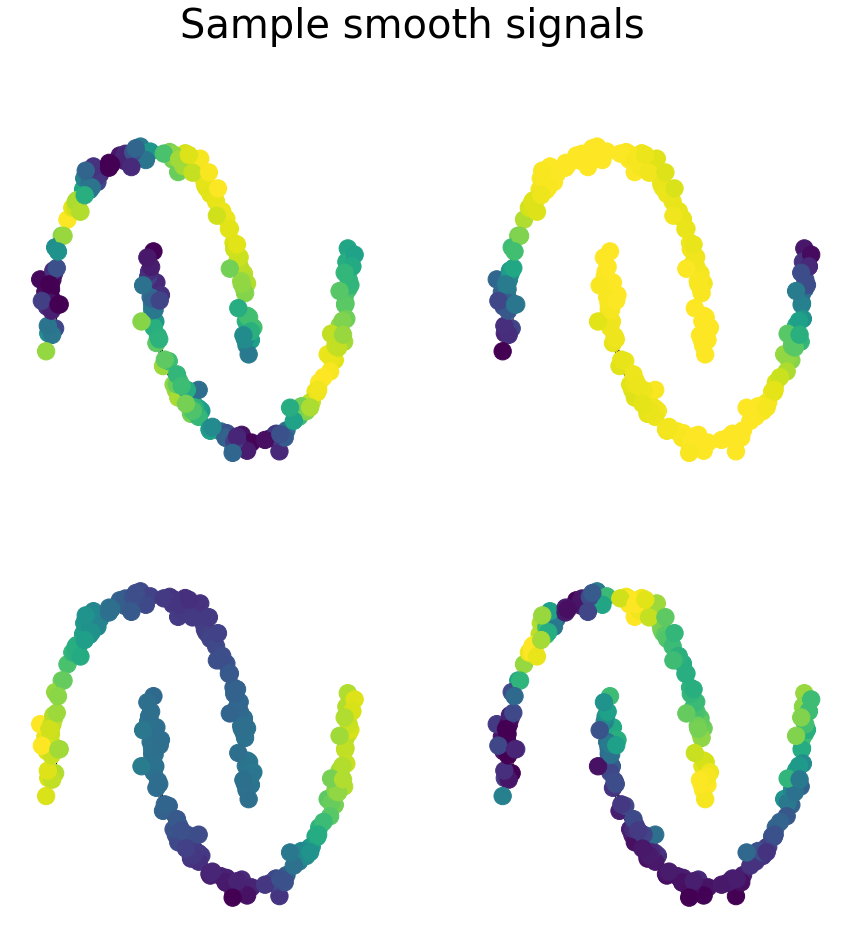
\includegraphics[width=0.5\textwidth]{images/p2/signals.png}\nl
\end{center}

Now we show the results for different $k$.

\begin{enumerate}
    \item $k = 0.05$
        \begin{center}
            % 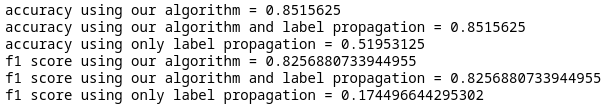
\includegraphics{images/p2/5_percent_stats.png}
            \begin{tabular}{|c|c|c|c|}
                \hline
                    & Our algorithm & Our algorithm and label propagation & Only label propagation\\
                \hline
                F1-score & 0.826 & 0.826 & 0.174 \\
                \hline
                Accuracy & 0.852 & 0.852 & 0.519 \\
                \hline
            \end{tabular}
        \end{center}
        \begin{center}
            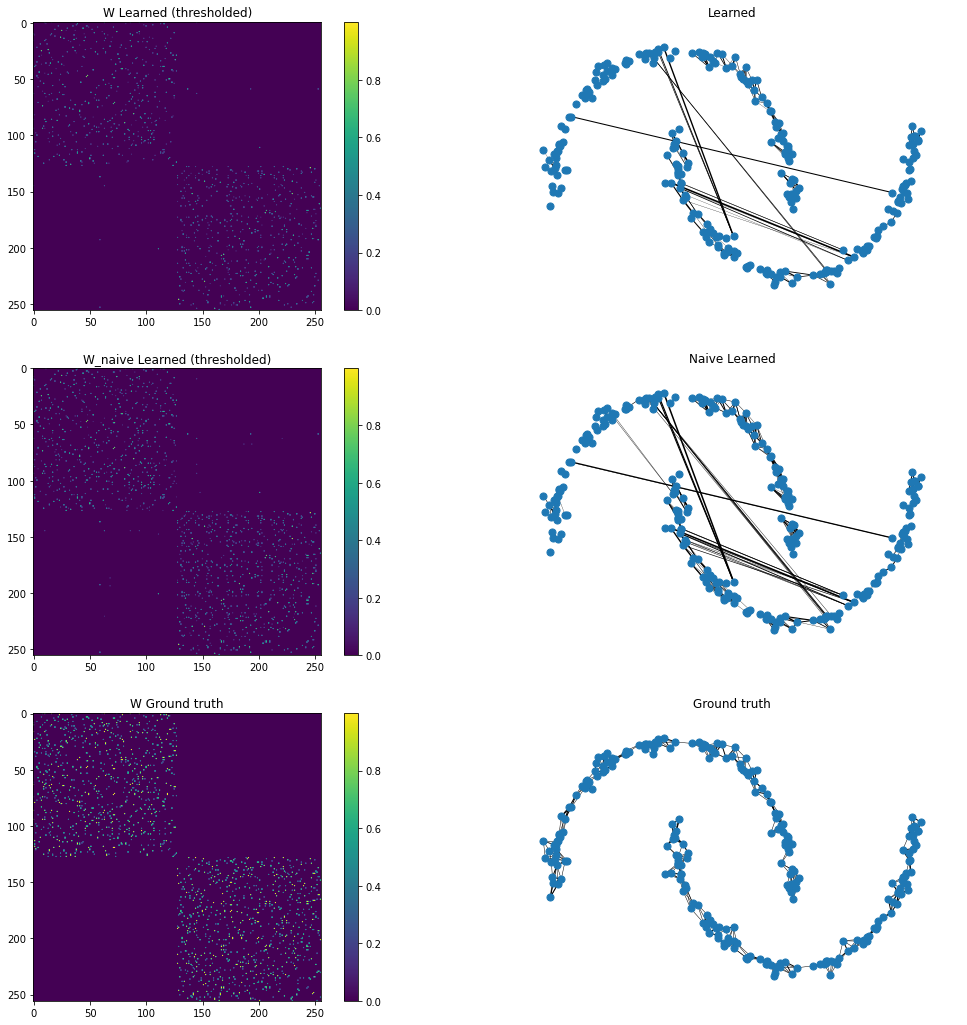
\includegraphics[width=0.75\textwidth]{images/p2/5_percent_learned_graphs.png}
        \end{center}
        \begin{center}
            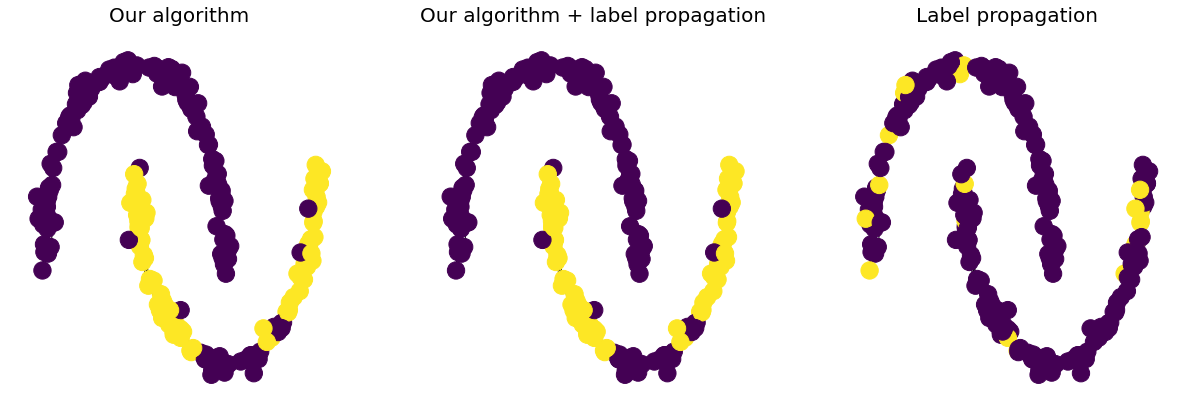
\includegraphics[width=0.75\textwidth]{images/p2/5_percent_predicted_labels.png}
        \end{center}
        \newpage
    \item $k = 0.1$
        \begin{center}
            % 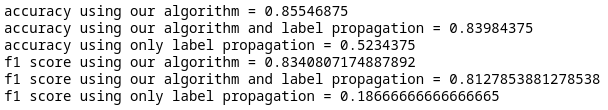
\includegraphics{images/p2/10_percent_stats.png}
            \begin{tabular}{|c|c|c|c|}
                \hline
                    & Our algorithm & Our algorithm and label propagation & Only label propagation\\
                \hline
                F1-score & 0.834 & 0.812 & 0.186 \\
                \hline
                Accuracy & 0.855 & 0.840 & 0.523 \\
                \hline
            \end{tabular}
        \end{center}
        \begin{center}
            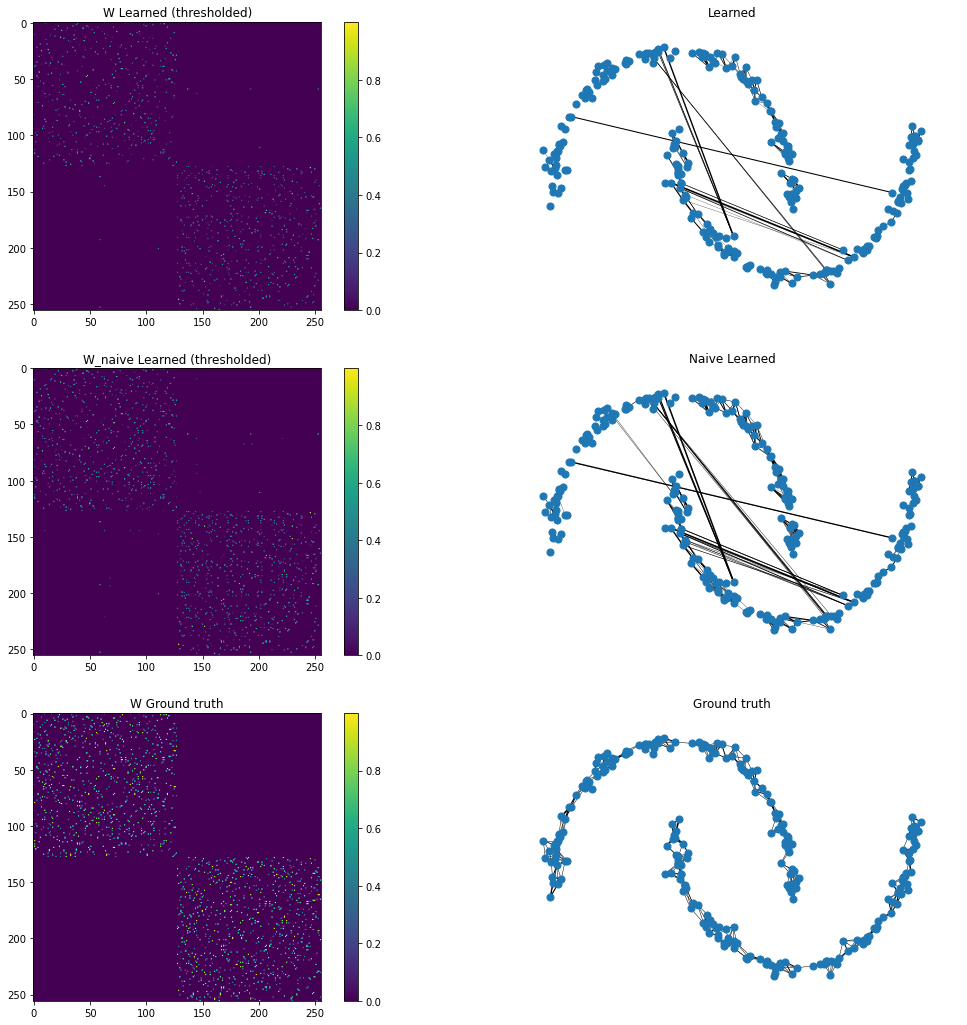
\includegraphics[width=0.75\textwidth]{images/p2/10_percent_learned_graphs.png}
        \end{center}
        \begin{center}
            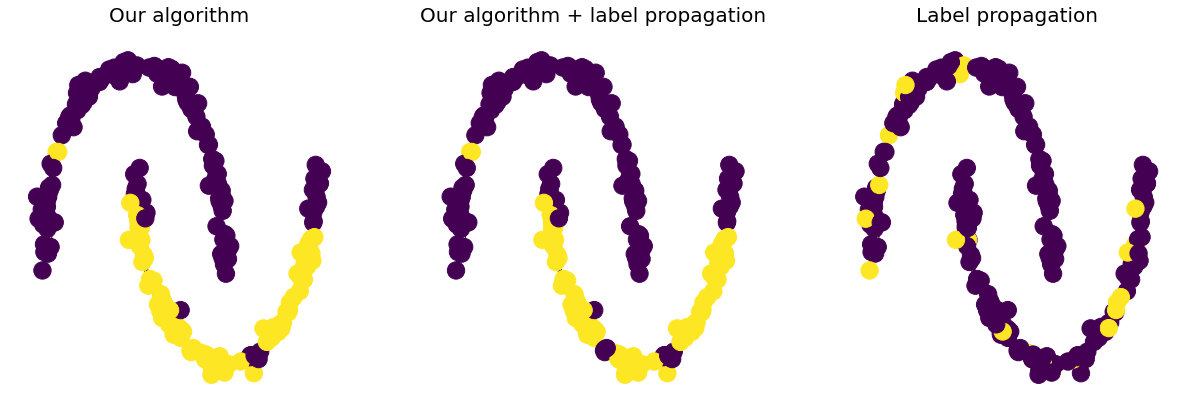
\includegraphics[width=0.75\textwidth]{images/p2/10_percent_predicted_labels.png}
        \end{center}
    \newpage

    \item $k = 0.2$
        \begin{center}
            % 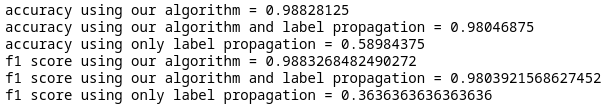
\includegraphics{images/p2/20_percent_stats.png}
            \begin{tabular}{|c|c|c|c|}
                \hline
                    & Our algorithm & Our algorithm and label propagation & Only label propagation\\
                \hline
                F1-score & 0.988 & 0.980 & 0.366 \\
                \hline
                Accuracy & 0.988 & 0.980 & 0.589 \\
                \hline
            \end{tabular}
        \end{center}
        \begin{center}
            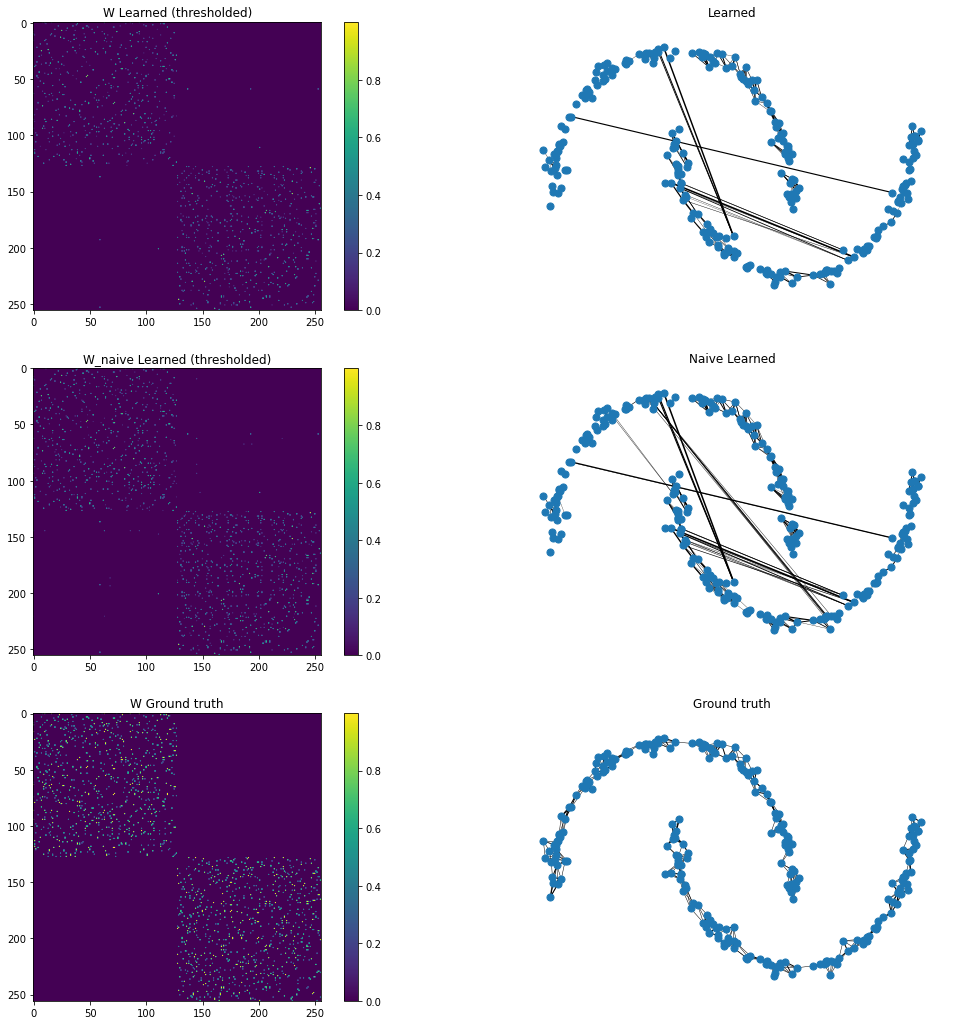
\includegraphics[width=0.75\textwidth]{images/p2/20_percent_learned_graphs.png}
        \end{center}
        \begin{center}
            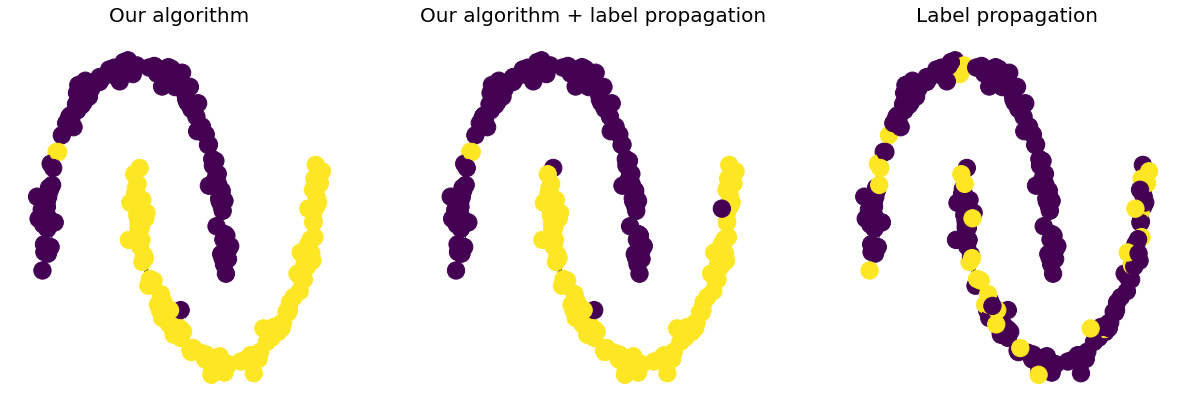
\includegraphics[width=0.75\textwidth]{images/p2/20_percent_predicted_labels.png}
        \end{center}

\end{enumerate}

\newpage

\section{Massive data setting}

\subsection{Problem}

Consider a massive data scenario, where $n$ and $d$ both are very large, and typically $n \gg d$. It is not possible to process the entire data every iteration. Explain how we can approach
the graph learning problem under such a setting. (Hint: Stochastic gradient descent based approaches try to address such problems, where each iteration is performed considering only a small
subset of the dataset, or a \emph{minibatch}).

\subsection{Solution}

The idea here will be similar to stochastic gradient descent. We will learn the graph in multiple iterations, and in each iteration, we shall randomly partition the set of vertices into blocks of size
$b > d$ (i.e., $b$ vertices in each block), and learn the induced subgraph for each block separately. Then we shall add the contributions of these induced graphs in the final weight matrix.\nl
Firstly, a note is in order. We are, for now, not picking these subgraphs in a very precise manner. After a few iterations of the above, we will have a sufficient amount of information in order to
fill the weight matrix $\mf{A}$ completely, and using this information, we can refine our choice of subgraphs as time progresses. Ideally we would like to be able to learn subgraphs that can be
embedded in a small neighbourhood (i.e., we roughly want to consider a subgraph where every vertex is in a certain distance of a certain vertex). We will look at it later.\nl
Now we will look at how the time complexity scales with the random approach.\nl
Suppose we have a block size of $b$. $b$ shouldn't be so small that there is no neighbourhood of a vertex to be learnt, and it shouldn't be so large that it would lead us to prohibitive time
or memory usage.\nl
Note that we process $n/b \times b(b - 1)/2$ edges in each iteration. So the probability that an edge $e = (v_i, v_j)$ is processed in one iteration is $p = \frac{b - 1}{n - 1}$. The probability
that there is at least one edge that is not processed after $k$ iterations is $(1 - p)^k$, so the probability that there is at least one vertex that is not processed is at most $\frac{n(n - 1)}{2}
(1 - p)^k$. So it would take
$\frac{n}{b} (2 \log n + c)$ iterations (for some constant $c$) to ensure that each edge has been processed (with a large enough probability). Let's suppose that learning the weight matrix takes time $f(n) \times n^2$. Then the time taken in an iteration
is $c \frac{n}{b} (2 \log n + c) \times \frac{n}{b} \times f(b) \times b^2 = f(b) \times n^2 (2 \log n + c)$. This gives us a speedup of $\frac{f(b) (2 \log n + c)}{f(n)}$ in cases where $f$ is linear. Since $f$ is
practically expected to be monotonically increasing, we will suffer a slowdown of at most $2 \log n + c$, which is not that bad. Even if $f(n) \approx \sqrt{n}$, we will have a net speedup in the
end for small enough $b$.\nl
Now as noted before, after we have already found a matrix $\mf{A}$ using this method (or with fewer iterations but ensuring that all edges have been covered at least once), we can do the
following: at each step, pick a vertex $v$ with the highest sum of weights that hasn't been chosen already (which can be a measure of how important the node is), and then pick $C > d$ of its neighbours such that the edges that join
them to $v$ have the highest weights. Do this recursively until you have reach a certain threshold on the number of nodes. And for these nodes, learn the subgraph and update $W$ accordingly. Now
once this has covered the entire graph, we can restart this process again and do this for a certain number of iterations until convergence.\nl
The justification on why this approach should work is as follows:
\begin{enumerate}
    \item For large graphs, where $n \gg d$, we can expect that the neighbourhood of a node should be small enough. This is due to the intuition that these vertices can be embedded in a low
        dimensional space. If we are allowed to make an assumption that most interactions concerning a vertex are fairly local, we expect this approach to work better too.
    \item In short, the algorithm tries to pick subgraphs that are roughly centered around important vertices. If there are no important vertices as such in the graph, then it is more or less equally
        likely for any vertex to be picked, so in the limit of a large number of iterations, we should expect a probability to be picked as the first node of the subgraph to be proportional
        to the sum of incident edge weights. For graphs where clustering is important, this will also try to take into account such clusters.
\end{enumerate}

\subsubsection{Experiment}

We will do two experiments here: the data will be synthetic here as well (and we will use the same method as done in problem 1). The idea will be the following:
\begin{enumerate}
    \item For a not-so-large dataset, compare the results of directly learning the underlying graph as well as the result of running the above algorithm (both variants: the one with random
        minibatches as well as the one where we also pick neighbourhoods of vertices).
\end{enumerate}

The dataset will be sensor networks again. We will look at the following cases with a given number of total passes over data:

\begin{enumerate}
    \item All the passes are allocated to the random batch picking (i.e., in this case we have no iterations of the guided type).
    \item Half the passes are allocated to the random batch picking and the other half to the guided type.
\end{enumerate}

For this example, we will use $N = 256$, $B = 64$, and $C = 20$ ($C$ chosen via hyperparameter tuning).\nl

\begin{center}
    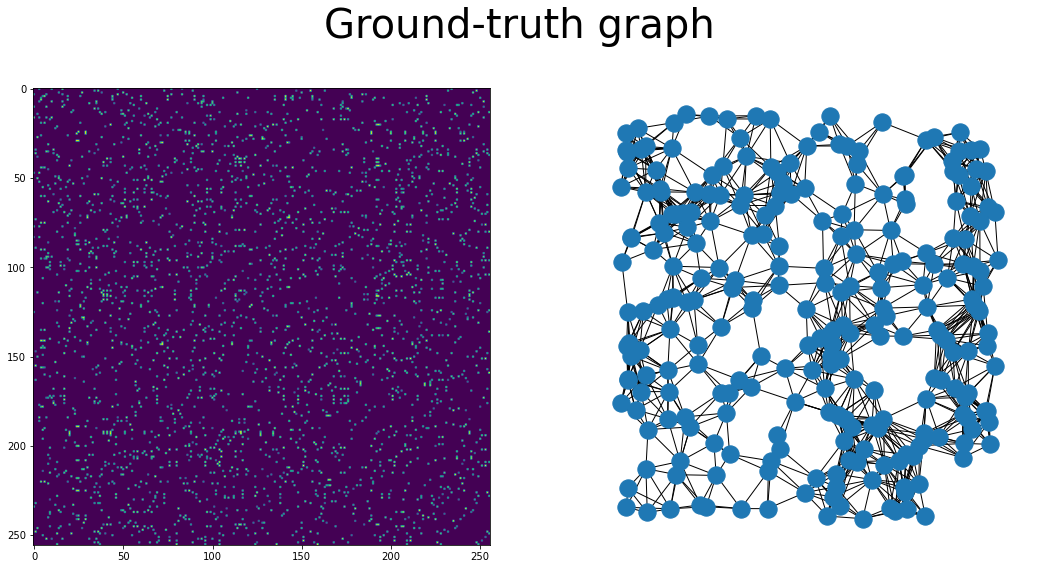
\includegraphics[width=0.7\textwidth]{images/p3/ground_truth_graph.png}\nl
    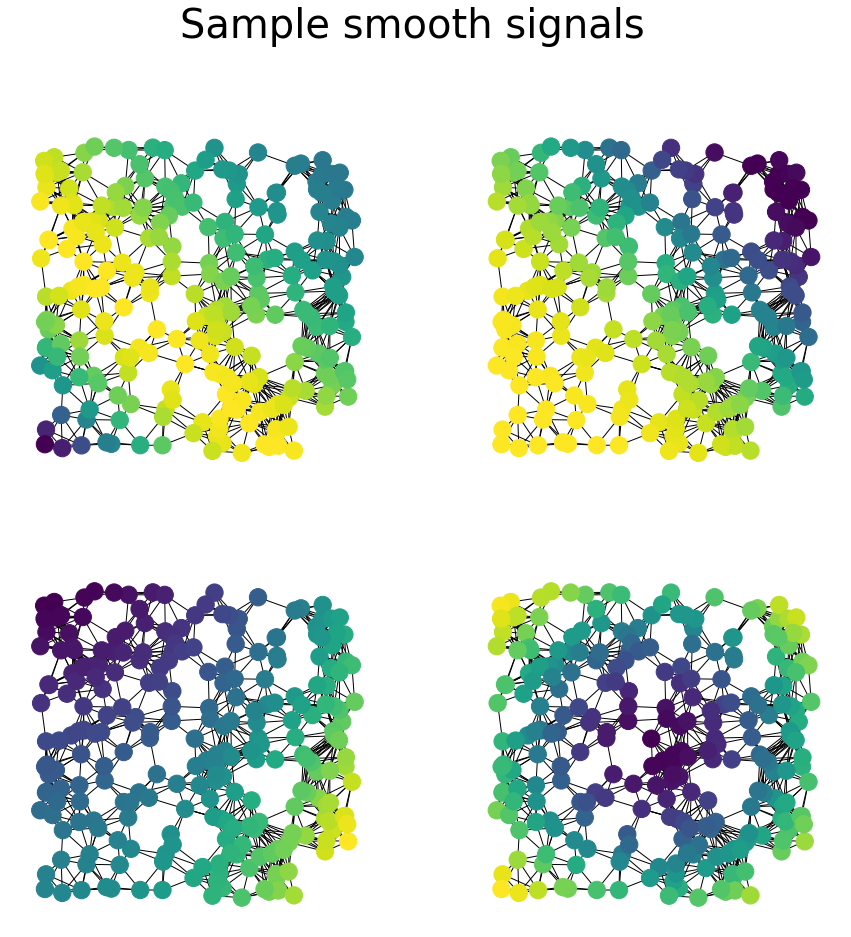
\includegraphics[width=0.7\textwidth]{images/p3/sample_smooth_signals.png}
\end{center}

\subsubsection{Results}

\begin{center}
    \begin{tabular}{|c|c|c|c|}
        \hline
            & No batch processing & Random batches & Random and guided batches\\
        \hline
        Edge existence F1-score & 0.70 & 0.71 & 0.74 \\
        \hline
    \end{tabular}
\end{center}

The following are the learned graphs and the spectra for
\begin{enumerate}
    \item Random batches:
        \begin{center}
            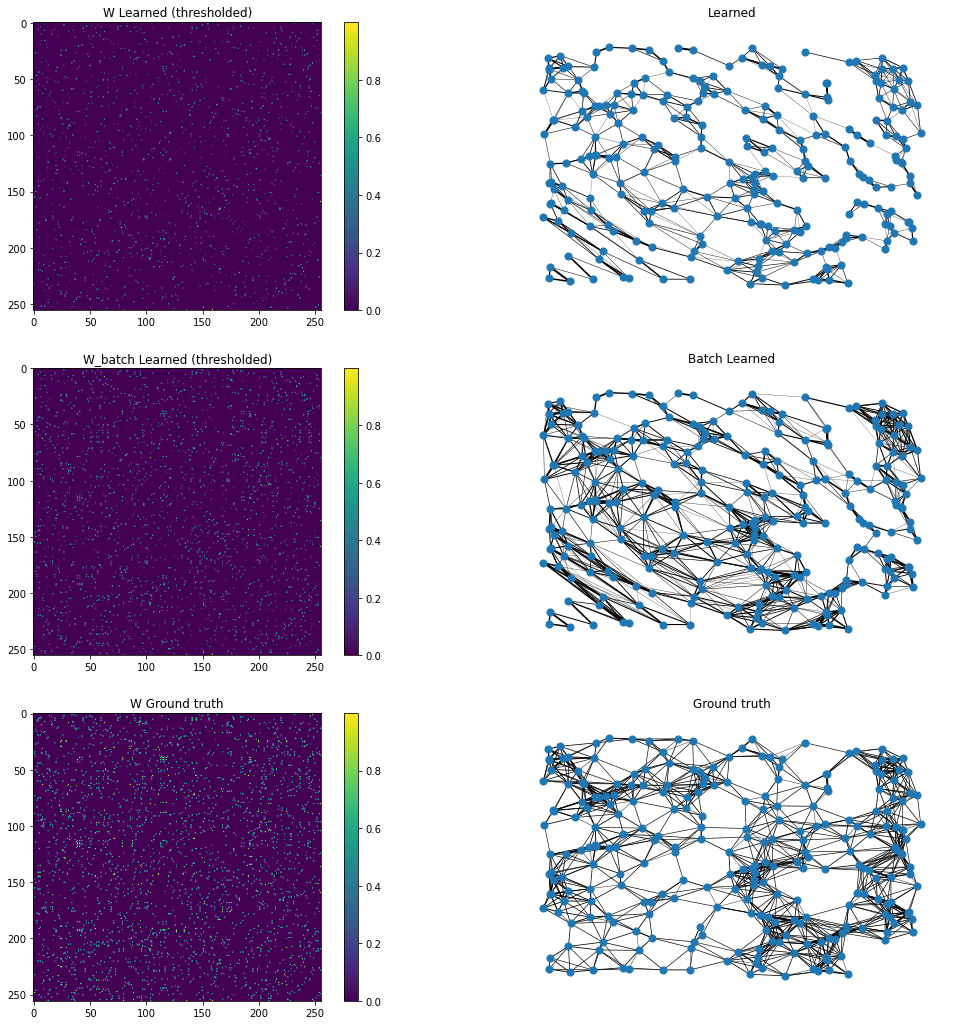
\includegraphics[width=0.9\textwidth]{images/p3/random_learned_graphs.png}\\
            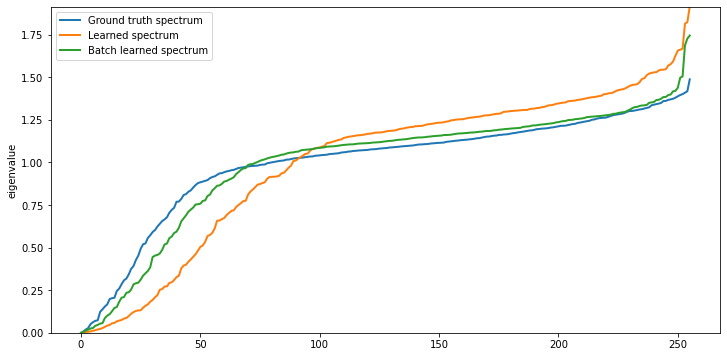
\includegraphics[width=0.9\textwidth]{images/p3/random_spectrum.png}
        \end{center}
    \item Random and guided batches:
        \begin{center}
            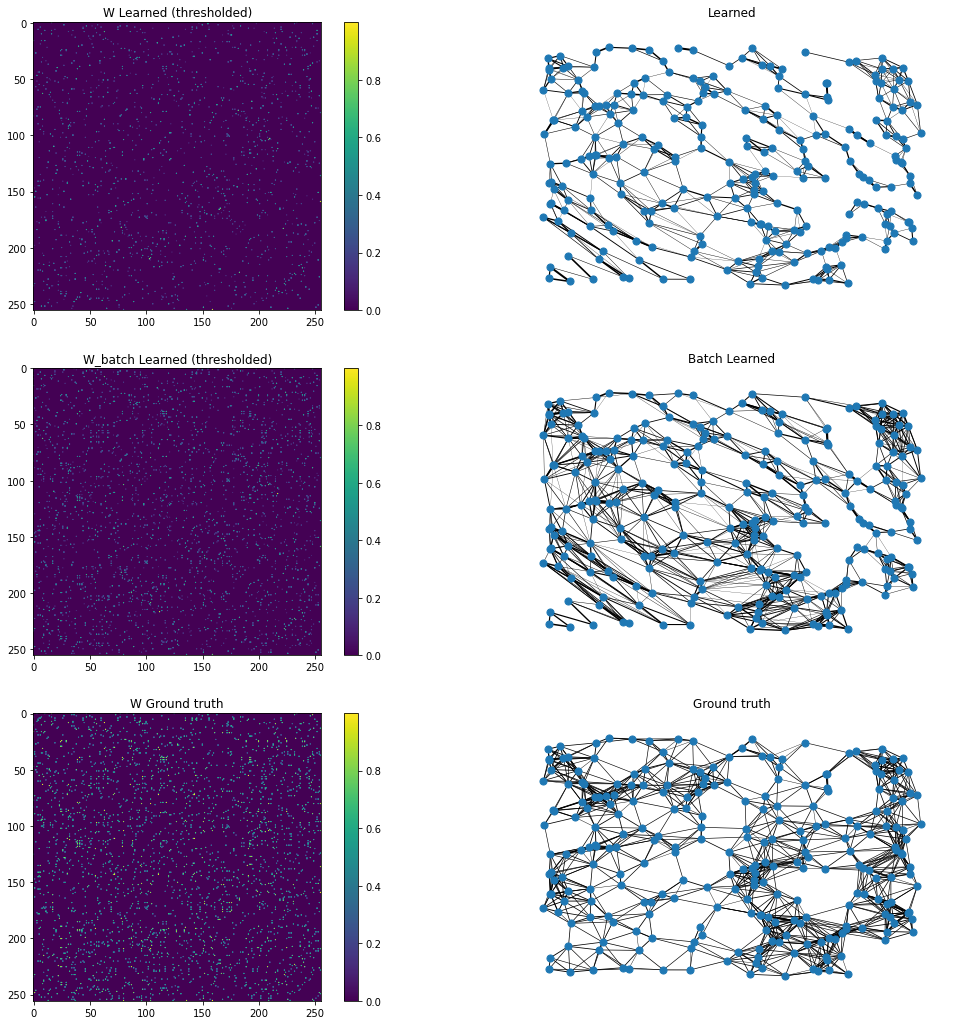
\includegraphics[width=0.9\textwidth]{images/p3/half_guided_learned_graphs.png}\\
            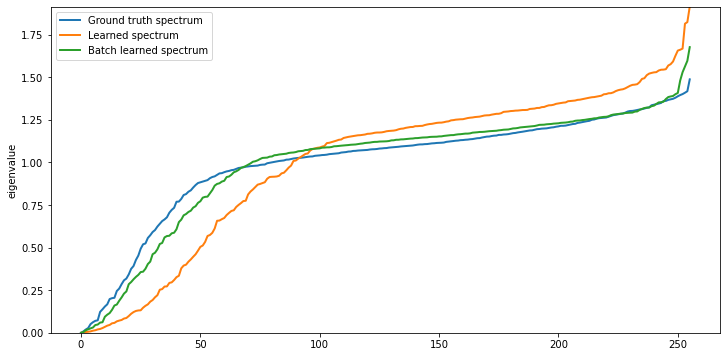
\includegraphics[width=0.9\textwidth]{images/p3/half_guided_spectrum.png}
        \end{center}
\end{enumerate}

Note that using a batch approach, we are also able to get a better fit to the spectrum of the ground-truth graphs (and a guided approach outperforms the random batch approach as well)
compared to the approach that learns the whole graph at once (however, this might just be specific to this dataset).\nl
More specifically, the L2 norm of vector of the differences between the eigenvalues
of the learned graph (without batches) and the ground-truth graph is $9.80$, for that between the random batch learned graph and the ground-truth graph is $1.32$, and for that between the guided
learned graph and the ground truth graph is $0.83$.

\newpage

\section{Heterogeneous data scenario}

\subsection{Problem}

Consider a heterogeneous data scenario, where the dataset $\mf{X}$ associated with vertices may belong to the set of reals $\R$, the set of integers $\mb{I}$, and categorical $\mb{C} = \{c_1,
\ldots, c_k\}$. More concretely, $\mf{X} \in \R^{n \times d_r} \times \mb{I}^{n \times d_i} \times \mb{C}^{n \times d_c}$ and $d = d_r + d_i + d_c$. For example, $\mf{x}_1 = [x_{11}, x_{12},
\ldots, x_{1d_r} \in \R, x_{1(d_r + 1)}, x_{1(d_r + 2)}, \ldots, x_{1(d_r + d_i)} \in \mb{I}, x_{1(d_r + d_i + 1)}, d_{1(d_r + d_i + 2)}, \ldots, x_{1(d_r + d_i + d_c)} \in \mb{C}]$. Explain in
detail how we can learn a graph matrix with heterogeneous data setting (in descriptive detail).

\subsection{Solution}

Building upon my answer to the second problem, we can note that for categorical features, we can apply the same ideas here as well. That is,
and add high penalties for weights of edges with endpoints belonging to different classes. It is not necessary to look at the ratios here, since we aren't trying to interpolate the features in
any manner, as they are given to us already.\nl
Now we need to also take care of integer data. I will make a crucial
assumption here (which should be taken care of before categorizing the data into integer and real data): all integer features represent data on a scale that we don't know about (and thus we can only talk
about their relative ranks rather than their actual magnitudes).\nl
This is because otherwise (for instance in the case where the feature corresponds to a count of something) we could have relaxed the
assumption that they were integers and used the standard formulation for reals instead. Some cases where this relaxation isn't justified is in the case where we have data from scales that
we can't quantify (for example, in a setting where the data consists of results of a questionnaire and the answer $1$ to a question corresponds to ``highly disagree'' while the answer $5$
corresponds to ``highly agree'').\nl
For such data, we can use some properties of their distribution rather than these values themselves, since only the ordering matters. In particular, properties like median and mode are much
more relevant in such a scenario. Hence, we will replace these features by their quantiles and then treat them as real features. This makes more sense, since in such an example, it makes more
sense to talk quantitatively about the difference between a person whose
response to a question lies at the $10$-th percentile, the $30$-th percentile, or the $50$-th percentile, rather than talk quantitatively about a person who answered $1$, $2$ or $3$.\nl

\subsubsection{Experiment}

Note that here synthetic data might not make the cut.
\todo{implement and add stuff}

\end{document}
